\documentclass[aspectratio=169]{beamer}
\usepackage[utf8]{inputenc}
\usepackage[T1]{fontenc}
\usepackage[french]{babel}
\usepackage{graphicx}
\usepackage{pgfpages}
\usepackage{amsmath}
\usepackage{amssymb}
\usepackage{mathtools}
\usepackage{xcolor}
\usepackage{prftree}

\graphicspath{{images/}}

% Theme pedagogique (identique a la lecon 1)
\usetheme{Boadilla}
\usecolortheme{seahorse}

% Activer les notes pour le presentateur
% \setbeameroption{show notes on second screen=right}

% Macros pour faciliter l'ecriture des regles de deduction
\newcommand{\blue}[1]{\textcolor{blue}{#1}}
\newcommand{\red}[1]{\textcolor{red}{#1}}
\newcommand{\oftype}{\mathrel{\red{:}}}

\title{Logique et Fondements de l'Informatique}
\subtitle{Logique propositionnelle \& Constructivisme}
\author{Pablo Donato}
\date{Leçon 2}

\begin{document}

% SLIDE 1 : Titre
\begin{frame}
  \titlepage
  \note{
    Bonjour à tous. Aujourd'hui, nous poursuivons notre exploration de Rocq en nous attaquant à la logique propositionnelle complète.\\
    Nous allons rajouter au connecteur de l'implication ($\to$) les connecteurs habituels : conjonction ($\land$), disjonction ($\lor$), absurdité ($\bot$), et négation ($\neg$).\\
    Je vous montrerai en même temps la syntaxe Rocq correspondante dans jsCoq.
  }
\end{frame}

% SLIDE 2 : Hook / Introduction
\begin{frame}{Logique Constructive et Interprétation BHK}
  \begin{columns}
    \begin{column}{0.55\textwidth}
      \textbf{Fondements de Rocq :}
      \begin{itemize}
        \item Calcul des Constructions Inductives (CoIC)
        \item Extension du $\lambda$-calcul
        \item Logique \textbf{constructive} (intuitionniste)
      \end{itemize}
      \vspace{0.3cm}
      \textbf{L'interprétation BHK (1930) :}
      \begin{itemize}
        \item Brouwer-Heyting-Kolmogorov
        \item Sémantique computationnelle % des connecteurs (retire pour economiser de la place)
      \end{itemize}
    \end{column}
    \begin{column}{0.45\textwidth}
      \begin{center}
        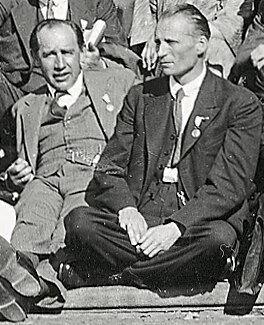
\includegraphics[height=2.6cm]{brouwer.jpg}
        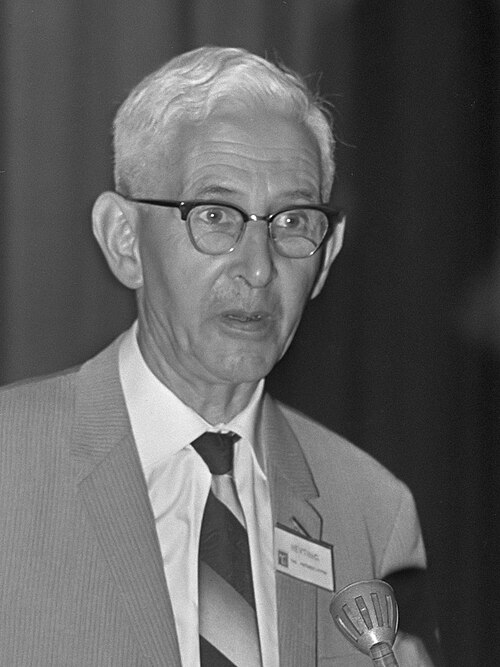
\includegraphics[height=2.6cm]{heyting.jpg} \\
        \vspace{0.1cm}
        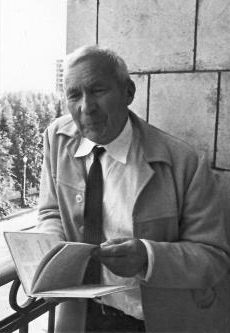
\includegraphics[height=2.6cm]{kolmogorov.jpg}\\
        \vspace{0.1cm}
        {\scriptsize L.E.J. Brouwer, A. Heyting, A. Kolmogorov}
      \end{center}
    \end{column}
  \end{columns}
  \note{
    Rappel : Via la correspondance de Curry-Howard, la logique naturellement supportée par Rocq est constructive. \\
    L'interprétation BHK donne un sens très concret, presque "algorithmique" à chaque connecteur. Aujourd'hui nous allons l'implémenter concrètement en étendant les termes du lambda-calcul.
  }
\end{frame}

% SLIDE 3 : Rappel Implication
\begin{frame}{Rappel : Implication ($\to$)}
  \begin{columns}
    \begin{column}{0.5\textwidth}
      \textbf{Introduction \only<2->{(Abstraction)} :}
      \[
        \alt<1>{
          \blue{\prftree[r]{${\to}I$}{\Gamma, A \vdash B}{\Gamma \vdash A \to B}}
        }{
          \blue{\prftree[r]{${\to}I$}{\Gamma, \red{x} \oftype A \vdash \red{M} \oftype B}{\Gamma \vdash \red{\lambda x.M} \oftype A \to B}}
        }
      \]
    \end{column}
    \begin{column}{0.5\textwidth}
      \textbf{Élimination \only<2->{(Application)} :}
      \[
        \alt<1>{
          \blue{\prftree[r]{${\to}E$}{\Gamma \vdash A \to B}{\Gamma \vdash A}{\Gamma \vdash B}}
        }{
          \blue{\prftree[r]{${\to}E$}{\Gamma \vdash \red{M} \oftype A \to B}{\Gamma \vdash \red{N} \oftype A}{\Gamma \vdash \red{M\ N} \oftype B}}
        }
      \]
    \end{column}
  \end{columns}
  \note{
    Commençons par un bref rappel. L'implication $A \to B$, c'est le type des fonctions de A vers B.\\
    L'introduction, c'est construire une fonction (lambda-abstraction).\\
    L'élimination, c'est utiliser cette fonction (application).
  }
\end{frame}

% SLIDE 4 : Implication (Detours)
\begin{frame}{Implication : Élimination des détours}
  \begin{center}
    \textbf{Principe de détours :}\\
    Introduire puis éliminer immédiatement est redondant.
  \end{center}

  % \vspace{0.2cm}
  % \textbf{Réduction de la dérivation complète :}
  % \vspace{0.2cm}
  $$
  \blue{
    \prftree[r]{${\to}E$}
    {\prftree[r]{${\to}I$}
      {\prfsummary{\Gamma, \red{x} \oftype A \vdash \red{M} \oftype B}}
    {\Gamma \vdash \red{\lambda x. M} \oftype A \to B}}
    {\prfsummary{\Gamma \vdash \red{N} \oftype A}}
    {\Gamma \vdash \red{(\lambda x.M)\ N} \oftype B}
  }
  \quad \boldsymbol{\rhd} \quad
  \blue{
    \prfsummary{\Gamma \vdash \red{M[N/x]} \oftype B}
  }
  $$

  \vspace{0.1cm}
  \begin{itemize}
    \item Substituer la preuve $u$ partout où l'hypothèse $x$ était requise dans $t$.
    \item Correspond exactement à la $\beta$-réduction du $\lambda$-calcul (semaine 2).
  \end{itemize}

  \note{
    Il est fondamental de comprendre ce qui se passe ici. La $\beta$-réduction n'est pas qu'un simple outil de calcul. C'est le retrait d'un détour logique ! Substituer la valeur à la place de la variable, c'est logiquement brancher la preuve concrète partout où l'hypothèse était exigée.
  }
\end{frame}

% SLIDE 5 : Conjonction (Regles)
\begin{frame}{Conjonction ($\land$)}
  \begin{columns}
    \begin{column}{0.45\textwidth}
      \textbf{Introduction \only<2->{(Paire)} :}
      \vspace{0.2cm}
      $$
      \alt<1>{
        \blue{\prftree[r]{${\land}I$}{\Gamma \vdash A}{\Gamma \vdash B}{\Gamma \vdash A \land B}}
      }{
        \blue{\prftree[r]{${\land}I$}{\Gamma \vdash \red{M} \oftype A}{\Gamma \vdash \red{N} \oftype B}{\Gamma \vdash \red{(M, N)} \oftype A \land B}}
      }
      $$
    \end{column}
    \begin{column}{0.55\textwidth}
      \textbf{Éliminations 1 \& 2 \only<2->{(Projections)} :}
      \vspace{0.2cm}

      $$
      \alt<1>{
        \blue{\prftree[r]{${\land}E_1$}{\Gamma \vdash A \land B}{\Gamma \vdash A}} \quad \blue{\prftree[r]{${\land}E_2$}{\Gamma \vdash A \land B}{\Gamma \vdash B}}
      }{
        \blue{\prftree[r]{${\land}E_1$}{\Gamma \vdash \red{M} \oftype A \land B}{\Gamma \vdash \red{\pi_1 M} \oftype A}} \quad \blue{\prftree[r]{${\land}E_2$}{\Gamma \vdash \red{M} \oftype A \land B}{\Gamma \vdash \red{\pi_2 M} \oftype B}}
      }
      $$
    \end{column}
  \end{columns}
  \note{
    En sémantique BHK, une preuve de "A et B", c'est une paire formée d'une preuve de A et d'une preuve de B.\\
    L'introduction de la conjonction crée donc une paire $(t, u)$.\\
    Les éliminations correspondent aux projections partielles : $\pi_1$ (qui extrait le premier élément) et $\pi_2$ (qui extrait le second).
  }
\end{frame}

% SLIDE 5 : Conjonction (Detours)
\begin{frame}{Conjonction : Élimination des détours}
  \begin{center}
    \textbf{Principe de détours ($\beta$-réduction étendue) :}\\
    Introduire puis éliminer immédiatement est redondant.
  \end{center}

  \vspace{0.5cm}
  \begin{columns}
    \begin{column}{0.5\textwidth}
      \textbf{Détour 1 :}
      $$
      \blue{
        \prftree[r]{${\land}E_1$}
        {\prftree[r]{${\land}I$}
          {\prfsummary{\Gamma \vdash \red{M} \oftype A}}
          {\prfsummary{\Gamma \vdash \red{N} \oftype B}}
        {\Gamma \vdash \red{(M, N)} \oftype A \land B}}
        {\Gamma \vdash \red{\pi_1(M, N)} \oftype A}
      }
      \ \boldsymbol{\rhd}\
      \blue{
        \prfsummary{\Gamma \vdash \red{M} \oftype A}
      }
      $$
    \end{column}
    \begin{column}{0.5\textwidth}
      \textbf{Détour 2 :}
      $$
      \blue{
        \prftree[r]{${\land}E_2$}
        {\prftree[r]{${\land}I$}
          {\prfsummary{\Gamma \vdash \red{M} \oftype A}}
          {\prfsummary{\Gamma \vdash \red{N} \oftype B}}
        {\Gamma \vdash \red{(M, N)} \oftype A \land B}}
        {\Gamma \vdash \red{\pi_2(M, N)} \oftype B}
      }
      \ \boldsymbol{\rhd}\
      \blue{
        \prfsummary{\Gamma \vdash \red{N} \oftype B}
      }
      $$
    \end{column}
  \end{columns}

  \note{
    Si je construis la paire $(t, u)$ pour prouver $A \land B$, puis que j'utilise tout de suite $\pi_1$ sur cette paire pour récupérer $A$ ... c'est un détour ! La preuve $t$ suffisait dès le départ. C'est calculatoirement équivalent à une étape d'évaluation.
  }
\end{frame}

% SLIDE 6 : Disjonction
\begin{frame}{Disjonction ($\lor$)}
  \textbf{Introduction 1 \& 2 \only<2->{(Injections)} :}
  $$
  \alt<1>{
    \blue{\prftree[r]{${\lor}I_1$}{\Gamma \vdash A}{\Gamma \vdash A \lor B}} \quad \blue{\prftree[r]{${\lor}I_2$}{\Gamma \vdash B}{\Gamma \vdash A \lor B}}
  }{
    \blue{\prftree[r]{${\lor}I_1$}{\Gamma \vdash \red{M} \oftype A}{\Gamma \vdash \red{\iota_1 M} \oftype A \lor B}} \quad \blue{\prftree[r]{${\lor}I_2$}{\Gamma \vdash \red{M} \oftype B}{\Gamma \vdash \red{\iota_2 M} \oftype A \lor B}}
  }
  $$

  \vspace{0.3cm}
  \textbf{Élimination \only<2->{(Raisonnement par cas)} :}
  \vspace{0.1cm}

  $$
  \alt<1>{
    \blue{\prftree[r]{${\lor}E$}{\Gamma \vdash A \lor B}{\Gamma, A \vdash C}{\Gamma, B \vdash C}{\Gamma \vdash C}}
  }{
    \blue{\prftree[r]{${\lor}E$}{\Gamma \vdash \red{M} \oftype A \lor B}{\Gamma, \red{x} \oftype A \vdash \red{N} \oftype C}{\Gamma, \red{y} \oftype B \vdash \red{P} \oftype C}{\Gamma \vdash \red{\text{match } M \text{ with } \iota_1 x \Rightarrow N \mid \iota_2 y \Rightarrow P \text{ end}} \oftype C}}
  }
  $$
  \note{
    Pour prouver $A \lor B$, il suffit de choisir l'un des deux (asymétrie constructiviste). Le terme conserve l'information du choix via l'injection $\iota_1$ ou $\iota_2$.\\
    L'élimination se fait via un "match" (filtrage par motif) : "si c'est $A$ je fais ceci, si c'est $B$ je fais cela".
  }
\end{frame}

% SLIDE 6 : Disjonction (Detours)
\begin{frame}{Disjonction : Élimination des détours}
  \textbf{Détour 1 (le cas de gauche) :}
  \vspace{0.1cm}

  \resizebox{0.95\textwidth}{!}{
    $
    \blue{
      \prftree[r]{${\lor}E$}
      {\prftree[r]{${\lor}I_1$}
        {\prfsummary{\Gamma \vdash \red{M} \oftype A}}
      {\Gamma \vdash \red{\iota_1 M} \oftype A \lor B}}
      {\prfsummary{\Gamma, \red{x} \oftype A \vdash \red{N} \oftype C}}
      {\prfsummary{\Gamma, \red{y} \oftype B \vdash \red{P} \oftype C}}
      {\Gamma \vdash \red{\text{match } \iota_1 M \text{ with } \iota_1 x \Rightarrow N \mid \iota_2 y \Rightarrow P \text{ end}} \oftype C}
    }
    \quad \boldsymbol{\rhd} \quad
    \blue{
      \prfsummary{\Gamma \vdash \red{N[M/x]} \oftype C}
    }
    $
  }

  \vspace{0.4cm}
  \textbf{Détour 2 (le cas de droite) :}
  \vspace{0.1cm}

  \resizebox{0.95\textwidth}{!}{
    $
    \blue{
      \prftree[r]{${\lor}E$}
      {\prftree[r]{${\lor}I_2$}
        {\prfsummary{\Gamma \vdash \red{M} \oftype B}}
      {\Gamma \vdash \red{\iota_2 M} \oftype A \lor B}}
      {\prfsummary{\Gamma, \red{x} \oftype A \vdash \red{N} \oftype C}}
      {\prfsummary{\Gamma, \red{y} \oftype B \vdash \red{P} \oftype C}}
      {\Gamma \vdash \red{\text{match } \iota_2 M \text{ with } \iota_1 x \Rightarrow N \mid \iota_2 y \Rightarrow P \text{ end}} \oftype C}
    }
    \quad \boldsymbol{\rhd} \quad
    \blue{
      \prfsummary{\Gamma \vdash \red{P[M/y]} \oftype C}
    }
    $
  }

  \note{
    Pareil pour la disjonction. Si on a introduit à gauche ($\iota_1$) et qu'on fait un match tout de suite, l'ordinateur peut simplifier instantanément parce qu'il sait exactement dans quelle branche on va tomber. Le calcul progresse.
  }
\end{frame}

% SLIDE 7 : Absurdite
\begin{frame}{L'Absurdité ($\bot$)}
  \begin{columns}
    \begin{column}{0.5\textwidth}
      \textbf{Introduction :}
      \begin{center}
        \emph{Aucune règle d'introduction.}
      \end{center}
      \vspace{0.5cm}
      En constructivisme, $\bot$ est défini comme le type vide (zéro constructeur).
    \end{column}
    \begin{column}{0.5\textwidth}
      \textbf{Élimination \only<2->{(Principe d'explosion)} :}
      \[
        \alt<1>{
          \blue{\prftree[r]{${\bot}E$}{\Gamma \vdash \bot}{\Gamma \vdash A}}
        }{
          \blue{\prftree[r]{${\bot}E$}{\Gamma \vdash \red{M} \oftype \bot}{\Gamma \vdash \red{\text{abort}(M)} \oftype A}}
        }
      \]
    \end{column}
  \end{columns}
  \note{
    L'absurdité ne se prouve jamais à partir de rien (heureusement). Sémantiquement, c'est le type sans aucun membre.\\
    Mais SI on a mystérieusement accès à une contradiction $\bot$, alors on peut déduire n'importe quoi ("ex falso quodlibet"). L'ordinateur offre alors le mot clé magique "abort" (ou un match vide) pour clore la branche actuelle.
  }
\end{frame}

% SLIDE 8 : Negation
\begin{frame}{La Négation ($\neg$)}
  \begin{center}
    \Large \textbf{La négation n'est pas primitive.}
  \end{center}
  \vspace{0.5cm}

  \textbf{Définition :}
  \[ \neg A \;\coloneqq\; A \to \bot \]

  \vspace{0.5cm}
  \begin{itemize}
    \item Prouver $\neg A$, c'est fournir une fonction qui transforme une preuve hypothétique de $A$ en contradiction.
    \item En Rocq : \texttt{not A} n'est qu'un ``sucre syntaxique'' pour \texttt{A -> False}.
  \end{itemize}
  \note{
    En constructivisme strict, nier $A$, c'est dire : "si tu me donnes $A$, je te construis une contradiction". La négation se manipule donc exactement avec les règles de l'implication : \texttt{intro} et \texttt{apply}. C'est une révélation souvent difficile pour les débutants.
  }
\end{frame}

% SLIDE 9 : Synthese
\begin{frame}{Synthèse : Bâtir avec Rocq}
  \begin{itemize}
    \item \textbf{Constructivisme concret :} Chaque connecteur possède une structure de \emph{données} ou de \emph{contrôle} associée.
    \item \textbf{Syntaxe Rocq (live) :}
      \begin{itemize}
        \item $\land$ $\rightarrow$ Paire (\texttt{split}, \texttt{destruct})
        \item $\lor$ $\rightarrow$ Type "somme" (\texttt{left}, \texttt{right}, \texttt{destruct})
        \item $\bot$ $\rightarrow$ Type \texttt{False} sans habitant (\texttt{exfalso})
        \item $\neg$ $\rightarrow$ Fonction retournant \texttt{False}
      \end{itemize}
  \end{itemize}
  \vspace{0.5cm}
  \begin{center}
    \emph{Passons maintenant à la pratique sur jsCoq !}
  \end{center}
  \note{
    On termine la théorie ici. Nous allons maintenant basculer sur l'interface jsCoq du navigateur, et taper les commandes correspondantes ensemble. C'est le moment d'allumer vos machines.
  }
\end{frame}

% SLIDE 10 : Bibliographie (Optionnelle si citee)
\begin{frame}[allowframebreaks]{Bibliographie}
  \nocite{troelstraHistoryConstructivism20th2011}
  \bibliographystyle{alphaurl}
  \bibliography{../../biblio}
\end{frame}

\end{document}
